\section{Superpixel}
\label{superpixel}

\todo{intro}

Eine \emph{Superpixelrepräsentation} eines Bildes $\gls{B}^{H \times W \times C}$ besteht aus einer Menge von $N \in \gls{N}$ \emph{Superpixeln} \bzw{} \emph{Regionen} $\gls{Smenge} \coloneqq {\left\{\gls{Smenge}_k\right\}}_{n=1}^N$ mit $\gls{Smenge}_n \subseteq W \times H$, sodass $\gls{Smenge}_i \cap \gls{Smenge}_j = \emptyset$ und $\bigcup\limits_{\gls{Smenge}_n \in \gls{Smenge}} \gls{Smenge}_n = W \times H$~\cite{super}.
Für eine gültige Superpixelsegmentierung fordern wir desweiteren, dass $\gls{Smenge}_n$ zusammenhängend ist~\cite{super}.
Aus der Menge an Superpixeln \gls{Smenge} lässt sich damit eine \emph{Segmentierungsmaske} $\gls{Smaske} \in {\left\{1, \ldots, N\right\}}^{H \times W}$ über
\begin{equation*}
  \gls{Smaske}_{yx} = n\,\, \text{\gdw{} } \left(x,y\right) \in \gls{Smenge}_n
\end{equation*}
gewinnen, die jedem Pixel in \gls{B} eine eindeutige Superpixelzugehörigkeit $n$ zuweist.

Aus einer Superpixelrepräsentation \gls{Smenge} \bzw{} \gls{Smaske} eines Bildes \gls{B} kann ein Graph im zweidimensionalen euklidischen Raum $\gls{G}=\left(\gls{V}, \gls{E}, \gls{p}\right)$ wie folgt definiert werden.
Seien dafür die einzelnen Superpixel $\gls{Smenge} = {\left\{\gls{Smenge}_n\right\}}_{n=1}^N$ die Knoten $\gls{V} = {\left\{\gls{v}_n\right\}}_{n=1}^N$ des Graphen \gls{G}, \dhe{} $\gls{v}_n = \gls{Smenge}_n$.
Die Positionsfunktion $\gls{p} \colon \gls{V} \to \gls{R}^2$ ordnet den einzelnen Superpixeln über
\begin{equation*}
  \gls{p}\left(\gls{v}_n\right) \coloneqq {\left[\bar{x}, \bar{y}\right]}^{\top} =  \frac{1}{\left|\gls{Smenge}_n\right|}\sum_{\left(x,y\right) \in \gls{Smenge}_n} {\left[x, y\right]}^{\top}
\end{equation*}
eine eindeutige Position in der Ebene über deren absoluten Schwerpunkt zu.
Die Kantenrelation \gls{E} des Graphen \gls{G} wird abschließend über die örtlichen Nachbarschaften der Superpixel basierend auf einem $3 \times 3$ Fenster um jeden Pixel in \gls{Smaske} definiert.
Falls sich \bspw{} die Werte in $\gls{Smaske}_{y+1,x}$ und $\gls{Smaske}_{y,x}$ unterscheiden,
\dhe{} $\gls{Smaske}_{y,x} \neq \gls{Smaske}_{y+1,x}$ mit $\gls{Smaske}_{y,x} = i$ und $\gls{Smaske}_{y+1,x}=j$, dann wird den Knoten $\gls{v}_i, \gls{v}_j \in \gls{V}$ über $\left(\gls{v}_i, \gls{v}_j\right) \in \gls{E}$ eine Kante in \gls{G} zugeordnet.
Formal lassen sich dabei erneut die zwei Konnektivitäten $4$ und $8$ unterscheiden, für die in der Praxis lediglich ein Unterschied in Bereichen erkennbar ist, deren Superpixelregionen rechteckig als Gitter aneinander liegen.
\begin{figure}[t]
\centering
\subfigure[Bild]{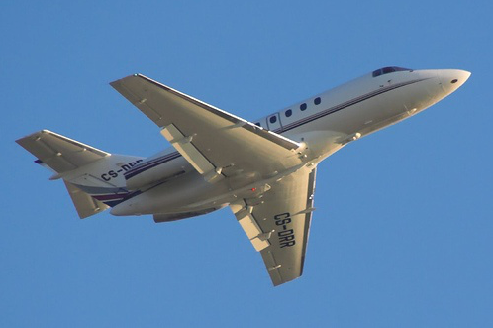
\includegraphics[scale=0.27]{bilder/flugzeug}}
\subfigure[Superpixelsegmentierung]{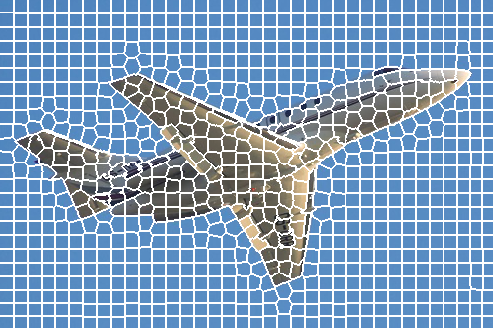
\includegraphics[scale=0.27]{bilder/flugzeug_slic}}
\subfigure[Graphrepräsentation]{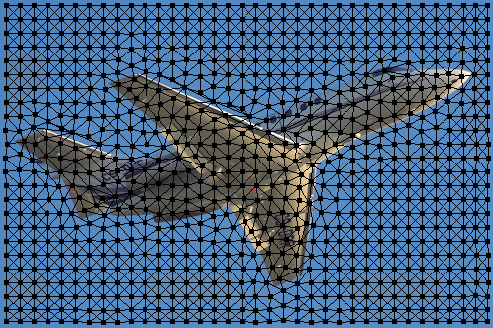
\includegraphics[scale=0.27]{bilder/flugzeug_slic_graph}}
\caption[Graphgenerierung aus einer Superpixelrepräsentation]{Illustration des Prozesses zur Graphgenerierung anhand einer Superpixelrepräsentation eines Bildes.
Ein Bild (a) wird dafür zuerst in eine Menge von Superpixeln segmentiert (b).
Die absoluten Zentren der Superpixel bilden die Knotenpunkte des Graphen.
Benachbarte Superpixel werden über eine Kante miteinander verbunden (c).}
\label{fig:superpixel_graph}
\end{figure}

Abbildung~\ref{fig:superpixel_graph} illustriert den beschriebenen Prozess der Graphgenerierung aus der Superpixelrepräsentation eines Bildes.

Zusätzlich zu der Positionsfunktion $p$ auf den Superpixelknoten kann der Graph \gls{G} um eine \emph{Massefunktion} $\gls{m} \colon \gls{V} \to \gls{N}$ mit $\gls{m}\left(\gls{v}_n\right) \coloneqq \left|S_n\right|$ zu $\gls{G} = \left(\gls{V}, \gls{E}, \gls{p}, \gls{m}\right)$ erweitert werden, die die Masse \bzw{} den Flächeninhalt der einzelnen Superpixelregionen beschreibt.

\paragraph{Globale und lokale Normierung}
\label{globale_lokale_normierung}

Eine Menge generierter Graphen aus den Superpixelrepräsentationen einer Bildermenge können sich zu Teilen extrem unterscheiden, \bspw{} durch variierende Auflösungen der Bilder.
So besitzt ein Graph möglicherweise nur sehr \enquote{kurze} Kanten, wohingegen ein anderer ausschließlich im Vergleich dazu aus \enquote{längeren} Kanten besteht.
Das kann bei der Transformation solcher Graphen in die Adjazenzmatrixrepräsentation $\gls{Adist} \in {\left[0, 1\right]}^{N \times N}$ aufgrund der Wahl des Parameters $\gls{sigma} \in \gls{R}$ zu Problemen führen.
Eine statische Wahl des Parameters \gls{sigma} führt dann \ggf{} zu Einträgen in \gls{Adist}, die stets sehr nahe bei Eins \bzw{} Null liegen.
Eine Normierung der Kantenlängen erscheint daher für die Transformation nach \gls{Adist} sinnvoll.
Eine \emph{Normierung} eines Graphen \gls{G} sieht dafür bei der Transformation nach \gls{Adist} eine Skalierung von ${\left\|\gls{p}\left(\gls{v}_i\right) - \gls{p}\left(\gls{v}_j\right)\right\|}_2^2 \in \gls{R}$ in das Intervall $\left[0, 1\right]$ vor.
Eine \emph{globale Normierung} von \gls{G} skaliert dabei ${\left\|\gls{p}\left(\gls{v}_i\right) - \gls{p}\left(\gls{v}_j\right)\right\|}_2^2$ über die maximale Kantenlänge ${\left\|\cdot\right\|}_2^2$ aller Kanten des Graphen, wohingegen die \emph{lokale Normierung} lediglich eine Skalierung über die maximale Kantenlänge der ausgehenden Kanten von $\gls{v}_i \in \gls{V}$ vorsieht.
Durch die lokale Normierung ist die Adjazenzmatrix \gls{Adist} insbesondere gerichtet.
Ein üblicher Trick, um dem entgegenzuwirken, ist die Aufsummierung von \gls{Adist} mit ihrer transponierten Matrix $\gls{Adist}^{\top}$ und der anschließenden Halbierung ihrer Werte, \dhe{} $\frac{1}{2}\left(\gls{Adist} + \gls{Adist}^{\top}\right)$~\cite{Reuter}.

Es ist anzumerken, dass der normierte Graph, repräsentiert als \gls{Adist}, neben der bereits vorhandenen Translationsinvarianz insbesondere skalierungsinvariant ist.
Im weiteren Verlauf dieser Arbeit wird der Prozess der Normierung eines Graphen implizit angenommen.

\paragraph{Effiziente Kantenbestimmung}
\label{kantenbestimmung}

Die Bestimmung der Kantenrelation \gls{E} kann aufgrund der Faltung über ein $3 \times 3$ Fenster recht teuer werden.
Ein eleganteres Verfahren

\subsection{Verfahren}
\label{superpixel_verfahren}

\paragraph{SLIC}
\label{slic}

\emph{\gls{SLIC}}~\cite{slic}

\paragraph{Quickshift}
\label{quickshift}

\cite{quickshift}

\paragraph{Weitere Verfahren}
\label{weitere_superpixel_verfahren}

In der Literatur finden sich zahlreiche weitere Verfahren zur Bestimmung einer Superpixelrepräsentation aus einem Bild mit jeweils unterschiedlichen Stärken und Schwächen~\cite{super, super2}.
While the past few years have seen considerable progress in eigenvector-based
methods of image segmentation, these methods are too slow to be
practical for many applications.~\cite{felzenszwalb}.
While there are other approaches to image segmentation that are highly efficient, these
methods generally fail to capture perceptually important non-local properties of an
image~\cite{felzenszwalb}.
Namenshaft zu erwähnen sei hier noch die \emph{effiziente graphbasierte Bildsegmentierung} von Felzenszwalb, in der Regel unter dem Namen \emph{Felzenszwalb-Segmentierung} bekannt~\cite{felzenszwalb}.
As with certain classical clustering methods, our method is based on
selecting edges from a graph, where each pixel corresponds to a node in the graph,
and certain neighboring pixels are connected by undirected edges. Weights on each
edge measure the dissimilarity between pixels. However, unlike the classical methods,
our technique adaptively adjusts the segmentation criterion based on the degree of
variability in neighboring regions of the image~\cite{felzenszwalb}

\subsection{Merkmalsextraktion}
\label{merkmalsextraktion}

Die Darstellung eines Bildes über einen Graphen \gls{G}, der aus einer Superpixelrepräsentation \gls{Smenge} gewonnen wurde, besitzt in der Regel weitaus weniger Knoten im Gegensatz zu der reinen Darstellung des Bildes über eine Gitterrepräsentation.
Die Superpixel \bzw{} die Regionen der Segmentierungsmaske können dabei die willkürlichsten Formen annehmen und besitzen lediglich die Einschränkung, dass diese stets zusammenhängend sind und keinerlei Löcher besitzen.
Die Form eines Superpixels muss demnach bestmöglichst eingefangen \bzw{} beschrieben werden können — ein Prozess, der in der Bildverarbeitung als \emph{Merkmalsextraktion} bekannt ist~\cite{momente}.
Ein geeigntes Mittel zur Beschreibung einzelner Objekte in einem segmentierten Bild sind die \emph{Momente}, welche in nicht-zentrierte, translationsinvariante, skalierungsinvariante und rotationsinvariante Momente unterschieden werden~\cite{momente}.

\paragraph{Nicht-zentrierte Momente}
\label{nicht_zentrierte_momente}

Zu einer binären Segmentierungsmaske $\gls{Smaske} \in {\left\{0, 1\right\}}^{Y \times X}$ sind die \emph{nicht-zentrierten Momente} vom Grad $\left(i+j\right)$, $i,j\in\gls{N}$, definiert als~\cite{momente}
\begin{equation*}
  \gls{M}_{ij} \coloneqq \sum_y^Y \sum_x^X y^i x^j \gls{Smaske}_{yx}.
\end{equation*}
Obwohl der Grad eines Moments beliebig hoch gewählt werden kann, so reichen in der Praxis meist wenige Momente niedrigen Grades aus ($\le 3$), um eine Region hinreichend genau zu charakterisieren~\cite{momente}.
Bildeigenschaften, die durch nicht-zentrierte Momente beschrieben werden können, sind unter anderem dessen Fläche über $\gls{M}_{00}$ sowie dessen absoluter Schwerpunkt $\left\{\bar{x}, \bar{y}\right\} = \left\{ \gls{M}_{01}/\gls{M}_{00}, \gls{M}_{10}/\gls{M}_{00}\right\}$~\cite{momente}.

\paragraph{Translationsinvariante (zentrale) Momente}
\label{translationsinvariante_momente}

Nicht-zentrierte Momente sind aufgrund ihrer Berücksichtigung der Position einer Region im Bild meist unerwünscht, sie helfen aber für die weitere Definition von translationsinvarianten Momenten.
Mit Hilfe der absoluten Schwerpunktskoordinaten $\left\{ \bar{x}, \bar{y} \right\}$ können die \emph{translationsinvarianten Momente} über
\begin{equation*}
  \gls{mu}_{ij} \coloneqq \sum_y^Y \sum_x^X {\left(y - \bar{y}\right)}^i {\left(x - \bar{x}\right)}^j \gls{Smaske}_{yx}.
\end{equation*}
definiert werden~\cite{momente}.
Sie lassen sich weiterhin direkt aus $\gls{M}_{ij}$ ermitteln.
So gilt \zB{}, dass $\gls{mu}_{00} = \gls{M}_{00}$ oder $\gls{mu}_{11} = \gls{M}_{11} - \bar{x}\gls{M}_{10} = \gls{M}_{11} - \bar{y}\gls{M}_{01}$ (\vgl{}~\cite{momente}).

\todo{index ändern}

\paragraph{Skalierungsinvariante Momente}
\label{skalierungsinvariante_zentrierte_momente}

\paragraph{Rotationsinvariante Hu-Momente}
\label{rotationsinvariante_momente}

\todo{kovarianzmatrix \bzw{} inertia tensor}

\cite{Siedhoff}
